%"/usr/texbin/lualatex" -interaction=nonstopmode %.tex|open %.pdf
\documentclass[10pt]{amsart}
\usepackage[T1]{fontenc}
\usepackage[utf8]{luainputenc}
\usepackage[english]{babel}

\usepackage{amsmath,amsthm,amssymb,stmaryrd,color,graphicx}
\usepackage{mathtools}
\usepackage{cmbright}
%\usepackage[onehalfspacing]{setspace}
\usepackage{setspace}
\usepackage{xspace}
\usepackage{longtable}
\usepackage{booktabs}
\usepackage{array}
\usepackage[protrusion=true,expansion=false]{microtype}
\usepackage{hyperref}
\usepackage[all]{xy}
\usepackage{sseq}

\usepackage{etoolbox}
\patchcmd{\subsubsection}{\itshape}{\bfseries}{}{}

\usepackage[natbib=true,style=numeric]{biblatex}
\usepackage[babel]{csquotes}
\bibliography{bibliography}

\usepackage{tikz}
\usetikzlibrary{arrows,shapes,trees,positioning,decorations.pathreplacing}

\theoremstyle{definition}
\newtheorem{defn}{Definition}[section]
\newtheorem{ex}[defn]{Example}
\theoremstyle{plain}
\newtheorem{prop}[defn]{Proposition}
\newtheorem{cor}[defn]{Corollary}
\newtheorem{lemma}[defn]{Lemma}
\newtheorem{thm}[defn]{Theorem}
\theoremstyle{remark}
\newtheorem{rem}[defn]{Remark}

\newcommand{\C}{\mathbb{C}}
\newcommand{\E}{\mathcal{E}}
\newcommand{\F}{\mathcal{F}}
\newcommand{\G}{\mathcal{G}}
\newcommand{\I}{\mathcal{I}}
\renewcommand{\O}{\mathcal{O}}
\newcommand{\U}{\mathcal{U}}
\newcommand{\Z}{\mathbb{Z}}
\newcommand{\Q}{\mathbb{Q}}
\newcommand{\N}{\mathbb{N}}
\newcommand{\R}{\mathbb{R}}
\newcommand{\PP}{\mathbb{P}}
\newcommand{\Ab}{\mathrm{Ab}}
\newcommand{\AbSh}{\mathrm{AbSh}}
\newcommand{\union}{\cup}
\newcommand{\intersection}{\cap}
\newcommand{\ev}{\mathrm{ev}}
\newcommand{\defeq}{\vcentcolon=}
\newcommand{\lra}{\longrightarrow}

\newcommand{\ie}{i.\,e.\@\xspace}
\newcommand{\eg}{e.\,g.\@\xspace}
\newcommand{\vs}{vs.\@\xspace}
\newcommand{\resp}{resp.\@\xspace}
\newcommand{\inv}{inv.\@\xspace}

\newcommand{\pt}{\mathrm{pt}}
\newcommand{\id}{\mathrm{id}}
\newcommand{\spot}{\underline{\ \ }}

\newcommand{\stackhref}[1]{\href{http://stacks.math.columbia.edu/tag/#1}{#1}}

\title{Higher direct images for dummies}

\author{Ingo Blechschmidt, Pascuale Zenobio De Rossi}

\date{\today}

\begin{document}

\begin{abstract}
Your abstract.
\end{abstract}

\maketitle

\section{Introduction}

\begin{itemize}
\item Give definitions of presheaves, sheaves, stalks.
\end{itemize}


\section{Locally constant sheaves}

\begin{itemize}
\item Give definition.
\item Explain sources of examples (and their usefulness): constant sheaves
(duh), direct images (sometimes), sheaves of solutions of differential
equations; and of course examples induced by covering spaces, representations
of the fundamental groupoid, and vector bundles with flat connection.
\item Explain the equivalence of locally constant sheaves and covering spaces;
also discuss how~$f^*$ and~$f_*$ look in this picture.
\item Explain the equivalence of locally constant sheaves and representations
of the fundamental groupoid. Calculate examples of the induced representation,
for instance with the sheaf~$\{ f \,|\, f' = \frac{1}{2z} f \}$
on~$\mathbb{C}^\times$ (which has monodromy~$f \mapsto -f$). Also explain how
to restrict on representations of the fundamental group at some fixed base
point (find out the technical hypotheses needed for this).
\item Explain the equivalence of locally constant sheaves and vector bundles
with flat connection. Warn that a visual representation of a vector bundles
necessarily lives in~$\mathbb{R}^3$ and thus, somewhat unfortunately, comes
with an induced connection.
\end{itemize}


\section{Direct images}

\begin{itemize}
\item Give the definition.
\item Explain how to easily calculate the stalks of the direct image in case
the map in question was closed. Explain how this is related to ``proper base
change''. Explain why closedness is intuitively necessary. Of course, give
\url{https://www2.math.uni-paderborn.de/fileadmin/Mathematik/People/wedhorn/Lehre/SkriptMannigfaltigkeiten.pdf}
as a reference.
\item Give description in terms of generators and relations (in the case that
this should turn out to be helpful).
\end{itemize}


\section{Sheaf cohomology and higher direct images}

\subsection{Basic definition and properties}

\begin{defn}Let~$\E$ be a sheaf of abelian groups on a topological space~$X$.
Then the \emph{$n$-th cohomology of~$X$ with values in~$\E$} is the abelian
group $H^n(X, \E) \defeq R^n\Gamma_X(\E)$, \ie the value of the~$n$-th right
derived functor of the global sections functor~$\Gamma_X : \AbSh(X) \to \Ab$.%
\footnote{A sequence of sheaves is exact if and only if the induced sequences of
stalks are exact, for all points of the space. It is a basic exercise in sheaf
theory to verify that~$\Gamma_X$ is always left-exact. The standard example of
an exact sequence which is not exact on global sections is the
\emph{exponential sequence} on~$\C \setminus \{0\}$, $0 \to \underline{\Z} \to \O \to
\O^\times \to 0$. Here~$\O$ denotes the sheaf of holomorphic functions and the
morphism~$\O \to \O^\times$ maps a holomorphic function~$f$ to~$\exp \circ f$.
This morphism is an epimorphism, since any nowhere vanishing holomorphic
function~$h$ can \emph{locally} be written as~$\exp \circ (\log \circ f)$,
where~$\log$ is some locally-existing branch of the complex logarithm. But the
induced map on global sections is not surjective. For instance, the function~$z
\mapsto 1/z$ has no preimage. To be a bit more dramatic: If the global sections
functor were exact, then the subject ``sheaf cohomology'' would not
exist.}
\end{defn}

Unrolling the definitions, the sheaf cohomology~$H^n(X,\E)$ is the cohomology
of the cochain complex~$\Gamma_X(\I^\bullet)$, where~$0 \to \E \to \I^0 \to \I^1
\to \cdots$ is a resolution of~$\E$ by injective objects. However, this
description is rarely useful in practice. We will discuss techniques for
calculating sheaf cohomology below.

\begin{ex}$H^0(X,\E) \cong \E(X)$.\end{ex}

\begin{ex}Sheaf cohomology on the one-point space~$\pt = \{ \heartsuit \}$ is
trivial, in the following sense:~$H^0(\pt,\E) \cong \E(\pt) \cong \E_\heartsuit$
and~$H^{\geq 1}(\pt,\E) = 0$ for any sheaf~$\E$. This is consistent with the
well-known vanishing of ordinary (singular or simplicial) cohomology on the
one-point space. An easy way to verify this is to note that~$\Gamma_\pt :
\AbSh(\pt) \to \Ab$ is exact (in fact, an equivalence of abelian categories).
This implies that the higher derived functors vanish.\end{ex}

With singular or simplicial cohomology, the choice of a coefficient ring does
not matter much in many applications; there is always the universal coefficient
theorem relating~$\Z$-valued cohomology with cohomology with values in other
rings. \emph{This is decidely not so with sheaf cohomology.} Sheaf cohomology
is as much about the topological space as it is about the sheaf in question.
The sheaf cohomology groups depend hugely on the used sheaf.

Unfortunately, there is no useful intuition about sheaf cohomology along the
ways of ``closed cochains modulo exact cochains''. Instead, some intuition on
what the elements of the sheaf cohomology groups look like can be gained by
Čech methods (see below).

The basic proposition about sheaf cohomology is that short exact sequences of
sheaves induce long exact sequences in cohomology.

\begin{prop}Let~$X$ be a topological space. Let~$0 \to \E \to \F \to \G \to 0$
be a short exact sequence of sheaves of abelian groups on~$X$. (This means that
the induced sequences~$0 \to \E_x \to \F_x \to \G_x \to 0$ on stalks are exact
for all points~$x \in X$.) Then there is a natural long exact sequence
\[ 0 \to \E(X) \to \F(X) \to \G(X) \to
  H^1(X,\E) \to H^1(X,\F) \to H^1(X,\G) \to H^2(X,\E) \to \cdots. \]
\end{prop}


\subsection{Relation to ordinary cohomology}

\begin{prop}Let~$X$ be a locally contractible space. Let~$R$ be a ring
and~$\underline{R}$ be the constant sheaf with stalks~$R$. Then
$H^\bullet_\text{sing}(X, R) \cong H^\bullet(X, \underline{R})$.
\end{prop}
\begin{proof}See~\cite{cibotaru}.
\end{proof}

\textbf{XXX}: Include comparison theorem with cohomology with values in local
systems.


\subsection{Why sheaf cohomology?}

Sheaf cohomology can be motived from many different angles.

\subsubsection*{The Leray spectral sequence} If~$f : X \to Y$ is any continuous map,
the cohomology of~$X$,~$Y$, and the fibers of~$f$ are related. The
Leray spectral sequence expresses this relationship in a precise way,
describing how the cohomology of~$X$ is composed by the cohomology of~$Y$ and
the cohomology of the fibers. However, even if one is only interested in the
cohomology of~$X$ with values in~$\Z$ or in a field, the cohomology of
non-constant sheaves appears in the spectral sequence. Only in special cases,
such that~$f$ is a fibration, does cohomology with values in local systems suffice.

\subsubsection*{Global sections} In complex and algebraic geometry, one is often
interested in the space of global sections of a sheaf~$\E$. For instance, in
the case that~$\E = \O_X(D)$ is the line bundle associated to a divisor~$D$ on a
complex manifold or scheme~$X$, $H^0(X,\E)$ is the space of meromorphic
functions on~$X$ with zeroes and poles behaviour governed by~$D$. However, this
space, or even its dimension, is hard to compute. Therefore one turns to the
\emph{Euler characteristic} of~$\E$, the alternating sum
\[ \chi(X,\E) \defeq \dim H^0(X,\E) - \dim H^1(X,\E) + \dim H^2(X,\E) \pm
\cdots \]
in which the global sections dimension appears as the first summand. This
quantity is in general easier to compute, since it is additive in short exact
sequences (if~$0 \to \E \to \F \to \G \to 0$ is exact, then~$\chi(X,\F) =
\chi(X,\E) + \chi(X,\G)$) and constant in certain families. Obviously,
sheaf cohomology is needed to define the Euler characteristic.

\subsubsection*{Classifying geometric objects} For certain choices of the sheaf, sheaf
cohomology classifies geometric objects. For instance, if~$X$ is a complex
manifold,~$H^1(X,\O_X^\times)$ classifies complex line bundles on~$X$ up to
isomorphism. Here,~$\O_X^\times$ is the sheaf of nowhere vanishing holomorphic
functions. More generally,~$H^1(X,\mathcal{A}ut(\E))$ classifies sheaves which
are locally isomorphic to a fixed sheaf~$\E$ and~$H^1(X,\G)$
classifies~$\G$-torsors on~$X$.

\subsubsection*{Irreducible spaces} The singular cohomology of irreducible topological
spaces -- spaces which cannot be written as the nontrivial union of two proper
closed subsets -- is always zero (in positive degrees). This is not a problem
when working with manifolds, which are irreducible only in the one-point case.
But it is a problem in algebraic geometry, where schemes with their Zariski
topology are often irreducible. For such cases, one is forced to look at
cohomology with values in non-constant sheaves.


\subsection{Higher direct images}

\begin{defn}Let~$f : X \to Y$ be a continuous map. Let~$\E$ be a sheaf of
abelian groups on~$X$. Then the \emph{$n$-th higher direct image of~$\E$
under~$f$} is the sheaf~$R^n f_*(\E)$ of abelian groups on~$Y$.\end{defn}

In this definition, $f_* : \AbSh(X) \to \AbSh(Y)$ denotes the left-exact
pushforward functor and~$R^n f_* : \AbSh(X) \to \AbSh(Y)$ denotes its~$n$-th right
derived functor.

\begin{ex}$R^0 f_*(\E) \cong f_*(\E)$.\end{ex}

\begin{ex}Sheaf cohomology is a special case of higher direct images: Let~$f : X
\to \pt$ be the unique map to the one-point space. Then~$H^n(X,\E) \cong R^n
f_*(\E)$ for any sheaf~$\E$ of abelian groups on~$X$.\end{ex}

For general maps~$f : X \to Y$, the higher direct image can be pictured as a
kind of ``relativized'' sheaf cohomology. To be more specific, we have the
following results.

\begin{prop}Let~$f : X \to Y$ be a continuous map. Let~$\E$ be a sheaf of
abelian groups on~$X$. Then~$R^n f_*(\E)$ is the sheafification of the
presheaf~$U \mapsto H^n(f^{-1}[U], \E)$ on~$X$.\end{prop}

\begin{proof}See \cite[Tag~\stackhref{01E4}]{stacks-project}.
\end{proof}

\begin{thm}[Proper base change theorem]\label{thm:proper-base-change}
Let~$X$ be a topological space such
that every open subspace is paracompact (\eg let~$X$ be a manifold). Let~$Y$ be
a Hausdorff space. Let~$f : X \to Y$ be a closed continuous map. Let~$\E$ be a
sheaf of abelian groups on~$X$. Then~$(R^n f_*(\E))_y \cong H^n(f^{-1}[y],
\E|_{f^{-1}[y]})$ for any point~$y \in Y$.\end{thm}

\begin{proof}See \cite[Thm.~8.11]{wedhorn}.\end{proof}

In the statement, the restriction~$\E|_{f^{-1}[y]}$ is defined as the pullback
of~$\E$ under the inclusion map~$i' : f^{-1}[y] \to X$ of the fiber in the
total space.

The proper base change theorem is very useful for visualizing the higher direct
image sheaves. The labeling ``base change'' is because the theorem can also be
formulated in the following way: Consider the pullback (fiber product) diagram
\[ \xymatrix{
  f^{-1}[y] \ar@{^{(}->}[r]^{i'} \ar[d]_{f'} & X \ar[d]^f \\
  \pt \ar@{^{(}->}[r]_i & Y.
} \]
Then $i^* R^n f_*(\E) \cong R^n f'_*(i'^*\E)$, since pulling back along~$i$ is
the same as calculating the stalk at~$y$ (example~\textbf{XXX}).

There is also a more general base change theorem, valid for maps~$i : Y' \to Y$
which are not necessarily the inclusion of a point.

\begin{ex}Let~$\id : X \to X$ denote the identity map. Since its fibers are
singletons, there should be no ``relative cohomology'' in positive degrees.
Indeed,~$R^n \id_*(\E)$ is zero for any sheaf~$\E$ and any~$n > 0$. This can be
verified directly with the definition (note that~$\id_* : \AbSh(X) \to
\AbSh(X)$ is the identity functor, which is exact). In case that the appropriate
topological hypotheses are satisfied, it also follows from the proper base
change theorem.\end{ex}

\textbf{XXX}: $R^q f_*(\E) = 0 \Rightarrow H^n(X,\E) \cong H^n(Y,f_*(\E))$.


\section{Čech methods}

\begin{defn}Let~$\E$ be a sheaf (or presheaf) of abelian groups on a
topological space~$X$. Let~$\U = (U_i)_i$ be an open covering. Then
\emph{the~$n$-th Čech cohomology of~$\E$ with respect to the covering~$\U$},
$\check H^n(\U,\E)$, is the~$n$-th cohomology group of the \emph{Čech cochain
complex~$\check C^\bullet(\U,\E)$}, which is defined as follows:
\[ \check C^n(\U,\E) \defeq \prod_{i_0,\ldots,i_n} \E(U_{i_0 \cdots i_n}), \]
where we set~$U_{i_0 \cdots i_n} \defeq U_{i_0} \cap \cdots \cap U_{i_n}$ and
use the differentials given by
\[ d ((s_{i_0 \cdots i_n})_{i_0 \cdots i_n}) \defeq
  \Bigl(\sum\nolimits_{k=0}^{n+1} (-1)^k \, s_{i_0 \cdots \widehat{i_k} \cdots
  i_{n+1}}|_{U_{i_0 \cdots i_{n+1}}}\Bigr)_{i_0 \cdots i_{n+1}}. \]
\end{defn}

Note that some people argue~\cite{nLab:cech} that Čech cohomology should not be
termed ``cohomology'', since it fails to satisfy the demands one has for true
cohomology theories (for instance, that short exact sequences induce long exact
sequences in cohomology). Rather, it should be regarded as a tool for computing
sheaf cohomology -- we will discuss their relation in due course.

Unlike with sheaf cohomology, calculating Čech cohomology is in principle a
viable linear algebra task. We can even restrict to the \emph{ordered Čech
complex}, given by
\[ \check C^n_{\text{ord}} = \prod_{i_0 < \cdots < i_n} \E(U_{i_0 \cdots i_n}),
\]
where~$I$ is endowed with some fixed total ordering and the differential is
given by the same formula. By an elementary result, this complex is homotopy
equivalent to the original one~\cite[Tag~\stackhref{01FG}]{stacks-project} and
has therefore isomorphic cohomology groups.


\subsection{The relation to sheaf cohomology}

Čech cohomology and sheaf cohomology are related by a spectral sequence, the
\emph{Čech-to-cohomology spectral sequence}.
\begin{prop}Let~$X$ be a topological space. Let~$\U = (U_i)_i$ be an open
covering of~$X$. Let~$\E$ be a sheaf of abelian groups on~$X$. Then there is a
spectral sequence with
\[ E_2^{pq} = \check H^p(\U, (U \mapsto H^q(U,\E))) \Longrightarrow
  H^{p+q}(X, \E). \]
\end{prop}
\begin{proof}See~\cite[Tag~\stackhref{01ES}]{stacks-project}.
\end{proof}

\begin{rem}The presheaf of which the Čech cohomology is taken in the
Čech-to-cohomology spectral sequence, $U \mapsto H^q(U,\E)$, is in general not
a sheaf. In fact, its sheafification is always
zero~\cite[Tag~\stackhref{03BA}]{stacks-project}.\end{rem}

In good cases, Čech cohomology does even agree with sheaf cohomology. This is
the content of \emph{Leray's theorem}.

\begin{prop}[Leray's theorem]Let~$X$ be a topological space. Let~$\U = (U_i)_i$ be an open
covering of~$X$. Let~$\E$ be a sheaf of abelian groups
on~$X$. Assume that~$\E$ is acyclic on the intersections~$U_{i_0 \cdots i_p}$,
that is~$H^q(U_{i_0 \cdots i_p}, \E) = 0$ for all~$p \geq 0$ and~$q > 0$.
Then~$H^n(X,\E) \cong \check H^n(\U,\E)$ for all~$n \geq 0$.\end{prop}

\begin{proof}The~$E_2$ page of the Čech-to-cohomology spectral sequence is
concentrated in the row~$q = 0$, since~$E_2^{pq}$ is a subquotient of~$\check
C^p(\U, H^q(\spot,\E))$, which is zero for~$q > 0$. Therefore the spectral
sequence degenerates. This implies the statement.
\end{proof}

The vanishing assumption of the theorem is usually not checked by hand, but a
result of \emph{vanishing theorems}. For instance, each of the following
conditions guarantees that~$H^n(X,\E)$ vanishes for all~$n > 0$:
\begin{itemize}
\item The space~$X$ is contractible and locally contractible, and~$\E$ is
constant. (In this case,~$H^n(X,\E)$ coincides with singular cohomology, for
which the vanishing is well-known.)
\item The space~$X$ is an affine scheme and~$\E$ is a
quasicoherent~$\O_X$-module. (This is \emph{Serre's vanishing theorem}.)
\item The space~$X$ is paracompact and the sheaf~$\E$ is flabby, fine, or soft.
Any sheaf of modules over the sheaf of continuous or smooth functions on a
manifold is fine.
\end{itemize}


\subsection{The Mayer--Vietoris sequence from a higher point of view}

\begin{prop}Let~$X = A \cup B$ be a covering of a topological space~$X$
by two open subsets. Let~$\E$ be a sheaf of abelian groups on~$X$. Then there
is a Mayer--Vietoris sequence
\[ \cdots \lra H^n(X, \E) \lra
  H^n(A, \E) \oplus H^n(B, \E) \lra
  H^n(A \cap B, \E) \stackrel{\partial}{\lra} H^{n+1}(X, \E) \lra \cdots. \]
\end{prop}
\begin{proof}Consider the Čech-to-cohomology spectral sequence for the
given open covering~$\U$. Since~$\U$ consists only of two open sets, its~$E_2$ page looks like this:
\begin{itemize}
\item $E_2^{pq}$ is zero for $p \geq 2$.
\item $E_2^{0q}$ equals the kernel of the map $H^q(A,\E) \oplus H^q(B,\E) \to H^q(A
\cap B,\E)$ which sends $(s,t)$ to $t|_{A \cap B} - s|_{A \cap B}$. (Use the
alternating Čech complex.)
\item $E_2^{1q}$ is the cokernel of that map.
\end{itemize}
Therefore the spectral sequence degenerates on the~$E_2$ page. Now
consider, for any $n \geq 0$, the canonical short exact sequence
\[ 0 \longrightarrow F^1 E_\infty^n \longrightarrow E_\infty^n
\longrightarrow E_\infty^n/F^1 E_\infty^n \longrightarrow 0. \]
Since~$F^2 E_\infty^n = F^3 E_\infty^n = \cdots = 0$ and~$F^0 E_\infty^n =
F^{-1} E_\infty^n = \cdots = E_\infty^n$ (by the vanishing of most
columns, see for instance~\cite{greenberg}),
we can express the outer terms of this sequence in~$E_2$ terms:
\[ 0 \longrightarrow E_2^{1,n-1} \longrightarrow E_\infty^n
\longrightarrow E_2^{0,n} \longrightarrow 0. \]
Explicitly, this is the sequence
\begin{align*}
  0 &\longrightarrow \mathrm{cok}(H^{n-1}(A) \oplus H^{n-1}(B) \to
H^{n-1}(A \cap B)) \\
  &\longrightarrow H^n(X) \\
  &\longrightarrow \mathrm{ker}(H^n(A) \oplus H^n(B) \to H^n(A \cap B)) \\
  &\longrightarrow 0.
\end{align*}
We can splice these short exact sequences to obtain the long exact
Mayer--Vietoris sequence.
\end{proof}

\begin{itemize}
\item Also give lemma that sheaf cohomology = singular cohomology. Again,
sketch the first step of the proof. Link to the very detailed reference
\url{http://www3.nd.edu/~lnicolae/sheaves_coh.pdf}. Also check out
\url{http://www.math.ru.nl/~mgroth/teaching/algtopII14/Section08.pdf} and
\url{http://mathoverflow.net/questions/4214/equivalence-of-grothendieck-style-versus-cech-style-sheaf-cohomology}.
\item Čech intuition for sheaf cohomology.
\item Direct limit over all coverings.
\item $\check H^0(\U,\E) = \E(X)$, if~$\E$ is a sheaf.
\item Special degrees 0, 1, and 2.
\item Special case: covering by a single open subset?
\end{itemize}



\section{The Leray spectral sequence}

\textbf{XXX}: Has to be moved to the correct place.

\begin{prop}Let~$f : X \to Y$ be a continuous map. Let~$\E$ be a sheaf of
abelian groups on~$X$. Then there is the \emph{Leray spectral sequence}
\[ E_2^{pq} = H^p(Y, R^q f_*(\E)) \Longrightarrow H^n(X, \E). \]
\end{prop}

\begin{proof}The mother of all spectral sequences is the spectral sequence
associated to a filtered complex. Her first child is the Grothendieck spectral
sequence; the Leray spectral sequence is a special case of it. Namely, the
composition
\[ \AbSh(X) \xrightarrow{f_*} \AbSh(Y) \xrightarrow{\Gamma_Y} \Ab \]
equals the global sections functor~$\Gamma_X$. Ignoring technicalities about
adapted classes, we obtain the Grothendieck spectral sequence
\[ E_2^{pq} = R^p\Gamma_Y(R^q f_*(\E)) \Longrightarrow R^n\Gamma_X(\E). \]
This is the Leray spectral sequence.
\end{proof}

\begin{ex}In the situation of the proposition, assume that the higher direct
images of~$\E$ vanish (\ie~$R^q f_*(\E) = 0$ for~$q > 0$). This is, for
instance, satisfied if the assumptions of the proper base change theorem
(Thm.~\ref{thm:proper-base-change}) are fulfilled and if~$\E$ has no higher
cohomology on the fibers of~$f$. Then the Leray spectral sequence degenerates
on the second page and shows that~$H^n(X,\E) \cong H^n(Y,f_*(\E)$.
\end{ex}


\section*{Locally constant sheaves}

\begin{ex}\label{twistarsch}
Consider $S^1$ together with the locally constant sheaf of typical stalk $\Z^2$ and monodromy representation $[\gamma].(a,b)=(b,a)$ where $[\gamma]$ is a generator of $\pi_1S^1$. We want to calculate its sheaf cohomology via cohomology with local coefficient system. The bundle of coefficients $E$ is given as $$E:=[0,1]\times\Z^2/\sim$$ with the identification $(0,(a,b))\sim (1,[\gamma].(a,b))=(1,(b,a))$ and the obvious projection $E\to S^1$. We want to apply the Mayer-Vietoris sequence to the standard decomposition $S^1=D^+\union D^-$ of $S^1$ into two open intervals yielding the exactness of
\[\begin{xy}
  \xymatrix{
  H^{k-1}(D^+,E)\oplus H^{k-1}(D^-,E)\ar[r] & H^{k-1}(D^+\intersection D^-,E)\ar[r] & H^k(S^1,E)\ar[r] & H^k(D^+,E)\oplus H^k(D^-,E)
  } 
  \end{xy}\]
On a simply connected space a local system of coefficients is globally constant and this shows that $H^k(S^1,E)=0$ for $k>1$. For $k=1$ the sequence becomes
\begin{align}\label{arsch}
\begin{xy}
  \xymatrix{
  H^0(D^+,E)\oplus H^0(D^-,E)\ar[r]\ar[d] & H^0(D^+\intersection D^-,E)\ar[r]\ar[d] & H^1(S^1,E)\ar[r] & 0\\
  \Z^2\oplus\Z^2\ar[r] & \Z^2\oplus\Z^2 & & 
  }
  \end{xy}
\end{align}
We have to identify the lower arrow.\newline
\begin{tikzpicture}[scale=1]
\draw (0,0) -- (10,0);
\draw (0,0.5) -- (0,-0.5);
\draw (0,0.5) -- (0.25,0.5);
\draw (0,-0.5) -- (0.25,-0.5);
\draw (10,0.5) -- (10,-0.5);
\draw (10,0.5) -- (9.75,0.5);
\draw (10,-0.5) -- (9.75,-0.5);
\draw (6,-0.5) arc (-30:30:1);
\draw (4,0.5) arc (150:210:1);
\draw (1,-0.5) arc (-30:30:1);
\draw (9,0.5) arc (150:210:1);
\draw [decorate,decoration={brace,amplitude=10pt},xshift=-5mm,yshift=42mm, rotate around={-90:(0,0)}]
(3.5,0.65) -- (3.5,6.5)node [black,midway,xshift=9pt] {\footnotesize
$\space$};
\draw [decorate,decoration={brace,amplitude=5pt},xshift=90mm,yshift=42mm, rotate around={-90:(0,0)}]
(3.5,0) -- (3.5,1)node [black,midway,xshift=9pt] {\footnotesize
$\space$};
\draw [decorate,decoration={brace,amplitude=10pt},xshift=105mm,yshift=-42mm, rotate around={90:(0,0)}]
(3.5,0.65) -- (3.5,6.5)node [black,midway,xshift=9pt] {\footnotesize
$\space$};
\draw [decorate,decoration={brace,amplitude=5pt},xshift=10mm,yshift=-42mm, rotate around={90:(0,0)}]
(3.5,0) -- (3.5,1)node [black,midway,xshift=9pt] {\footnotesize
$\space$};
\draw [->] (7,3) arc (100:140:120pt);
\draw [->] (8,3) arc (60:25:100pt);
\draw (7.5,3) node {$D^+$};
\draw [->] (4,-3) arc (270:220:120pt);
\draw [->] (5,-3) arc (270:340:60pt);
\draw (4.6,-3) node {$D^-$};
\draw[fill=black] (0.5,0) circle (0.1);
\draw[fill=black] (5,0) circle (0.1);
\draw (0.5,0.5) node {$0.1$};
\draw (5,0.5) node {$0.5$};
\draw (11,0) node {$S^1$};
\end{tikzpicture}\newline
For an arbitrary space $X$ a cochain representing a class in $H^0(X,E)$ assigns to every point $x\in X$ a value in the corresponding fibre $E_x$. The cochain condition means that this value is constant on connected components of $X$. There are no nontrivial coboundaries in this dimension. Therefore we have a very clear understanding of how the groups in the diagram \ref{arsch} are isomorphic to $\Z^k$ namely by evaluation at some fixed points:
\begin{align}\label{arsch2}
  \xymatrix{
  H^0(D^+,E)\oplus H^0(D^-,E)\ar[r]\ar[d]_{\ev_{0.5}}^{\ev_{0.5}} & H^0(D^+\intersection D^-,E)\ar[r]\ar[d]^{\ev_{0.1}\oplus\ev_{0.5}} & H^1(S^1,E)\ar[r] & 0\\
  \Z^2\oplus\Z^2\ar[r] & \Z^2\oplus\Z^2 & & 
  }
\end{align}
Consider the cohomology class in $H^0(D^+,E)$ represented by the cocycle which maps $0.5\mapsto (a,b)\in\Z^2$. This cocycle restricted to $D^+$ also maps $0.1$ to $(a,b)$ because both of these points lie in the same connected component of $D^+$. Thus under isomorphisms \ref{arsch2} the restriction homomorphism $H^0(D^+,E)\to H^0(D^+\intersection D^-,E)$ maps $(a,b)\mapsto ((a,b),(a,b))$.
On the other hand the cohomology class in $H^0(D^-,E)$ represented by the cocycle which maps $0.5\mapsto (c,d)\in\Z^2$ maps $0.1\mapsto (d,c)$ since we have to let the monodromy act first. Therefore the restriction homomorphism $H^0(D^-,E)\to H^0(D^+\intersection D^-,E)$ maps $(c,d)\mapsto ((d,c),(c,d))$.
Mere calculation shows that the cokernel of $H^0(D^+,E)\oplus H^0(D^-,E)\to H^0(D^+\intersection D^-,E)$ is isomorphic to $\Z$ yielding $$H^1(S^1,E)\cong\Z\text{.}$$
\end{ex}


\section*{Direct Images}
\begin{ex}\label{twosheet}
Consider the $2$-sheeted covering $p:S^1\to S^1,z\to z^2$ viewing $S^1\subset\C$. We want to describe the direct image $p_*\underline{\Z}$ of the constant sheaf $\underline{\Z}$. The sheaf $p_*\underline{\Z}$ is locally constant hence it is determined by its monodromy representation $\pi_1S^1=\Z\curvearrowright\Z^2$. The curve $\gamma:[0,2\pi]\to S^1, t\mapsto\exp(i t)$ is a generator of $\pi_1S^1$ and we want to find a lift of this curve $I\to p_*\underline{\Z}$ to the étalé space of $p_*\underline{Z}$ with any given initial condition $\tilde{\gamma}(0)\in p_*\underline{\Z}_0$:

$$\begin{xy}
  \xymatrix{
  & p_*\underline{\Z}\ar[d]^{\pi}\\
  I\ar[r]_{\gamma}\ar[ru]^{\tilde{\gamma}} & S^1
  }
\end{xy}$$
\end{ex}
We choose two trivialisations
$$\begin{xy}
  \xymatrix{
p_*\underline{\Z}S^1\setminus\{+1\}=\underline{\Z}p^{-1}S^1\setminus\{+1\}=\underline{\Z}S^1\setminus\{\pm 1\}\ar[r]^/1.25cm/{\phi} & \Z_{upper}\oplus\Z_{lower}\\
p_*\underline{\Z}S^1\setminus\{-1\}=\underline{\Z}p^{-1}S^1\setminus\{-1\}=\underline{\Z}S^1\setminus\{\pm i\}\ar[r]^/1.25cm/{\psi} & \Z_{left}\oplus\Z_{right}
  }
\end{xy}$$
where for instance one generator of $\Z_{upper}$ corresponds to the locally constant real-valued function taking the value $+1$ on the upper connected arc of $S^1\setminus\{\pm 1\}$ and vanishing on the lower one.\newline

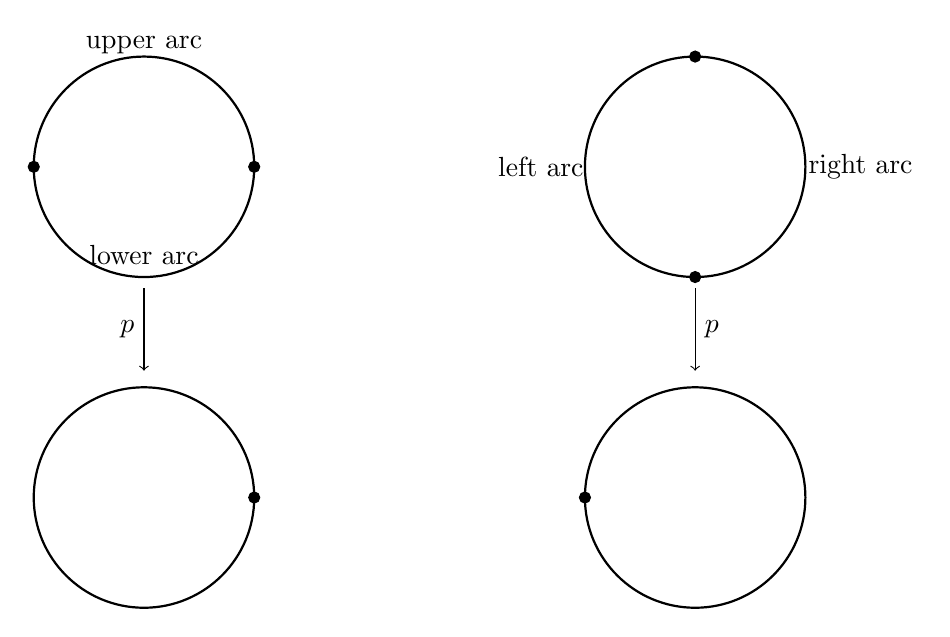
\begin{tikzpicture}[scale=0.7]
\draw[style=thick] (2,0) circle (2);
\draw[fill=black] (0,0) circle (0.1);
\draw[fill=black] (4,0) circle (0.1);
\draw[style=thick] (2,-6) circle (2);
\draw[fill=black] (4,-6) circle (0.1);
\draw[->] (2,-2.2) -- (2,-3.7) node[pos=.5,left] {$p$};

\draw[style=thick] (12,0) circle (2);
\draw[fill=black] (12,2) circle (0.1);
\draw[fill=black] (12,-2) circle (0.1);
\draw[style=thick] (12,-6) circle (2);
\draw[fill=black] (10,-6) circle (0.1);
\draw[->] (12,-2.2) -- (12,-3.7) node[pos=.5,right] {$p$};

\draw (2,2.2) node {upper arc};
\draw (2,-1.6) node {lower arc};
\draw (9.2,0) node {left arc};
\draw (15,0) node {right arc};
\end{tikzpicture}

%FICKEN, IST TIKZ ÄTZEND!!!

\vspace{1cm}

Let us describe the lift $\tilde{\gamma}$ with the initial condition $\tilde{\gamma}(0)=[\psi^{-1}(1,0)]_1$. At time $t=\pi-\varepsilon$ this lift still has the value $[\psi^{-1}(1,0)]_{\gamma(\pi-\varepsilon)}$ and we claim:
\begin{align}
\tilde{\gamma}(\pi-\varepsilon)&=[\psi^{-1}(1,0)]_{\gamma(\pi-\varepsilon)}\\
&=[\phi^{-1}(0,1)]_{\gamma(\pi-\varepsilon)}\label{claim}
\end{align}
The point $\tilde{\gamma}(\pi-\varepsilon)$ is obtained as follows: consider the locally constant real-valued function $f\in p_*\underline{\Z}(S^1\setminus\{-1\})=\underline{\Z}(S^1\setminus\{\pm i\})$ having the value $1$ on the left arc and $0$ on the right one. This is a section of $p_*\underline{\Z}$ over the open set $S^1\setminus\{-1\}$. The preimage of $\gamma(\pi-\varepsilon)$ consists of the two points $\exp\left(\frac{i(\pi-\varepsilon)}{2}\right)$ and $\exp\left(\frac{i(3\pi-\varepsilon)}{2}\right)$:\vspace{1cm}
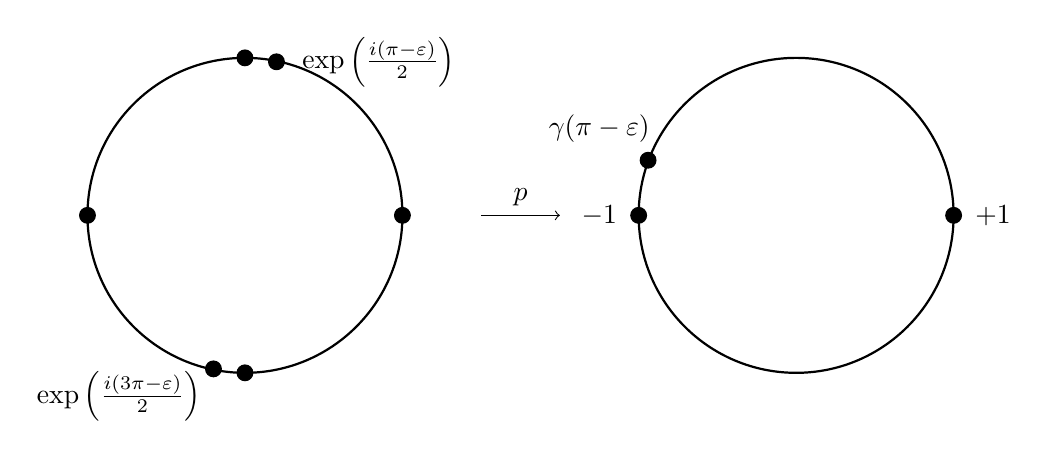
\begin{tikzpicture}[scale=1]
\draw[style=thick] (2,0) circle (2);
\draw[fill=black] (0,0) circle (0.1);
\draw[fill=black] (4,0) circle (0.1);
\draw[fill=black] (2,2) circle (0.1);
\draw[fill=black] (2,-2) circle (0.1);
\draw[fill=black] (2.4,1.95) circle (0.1);
\draw[fill=black] (1.6,-1.95) circle (0.1);
\draw[fill=black] (7,0) circle (0.1);
\draw[fill=black] (11,0) circle (0.1);
\draw[fill=black] (7.12,0.7) circle (0.1);
\draw (6.5,1.1) node {$\gamma(\pi-\varepsilon)$};
\draw[style=thick] (9,0) circle (2);
\draw[->] (5,0) -- (6,0) node[pos=0.5,above] {$p$};
\draw (6.5,0) node {$-1$};
\draw (11.5,0) node {$+1$};
\draw (3.7,1.95) node {$\exp\left(\frac{i(\pi-\varepsilon)}{2}\right)$};
\draw (0.4,-2.3) node {$\exp\left(\frac{i(3\pi-\varepsilon)}{2}\right)$};
\end{tikzpicture}\newline
On the other hand the real-valued function $g:=\phi^{-1}(0,1)\in p_*\underline{\Z}(S^1\setminus\{+1\})=\underline{\Z}(S^1\setminus\{\pm 1\})$ having the value $0$ on the upper arc and $1$ on the lower one represents exactly the same stalk of $p_*\underline{\Z}$ at the point $\gamma(\pi-\varepsilon)$. This proves claim (\ref{claim}).

A similar argument shows
\begin{align*}
\tilde{\gamma}(2\pi-\varepsilon)&=[\phi^{-1}(0,1)]_{\gamma(2\pi-\varepsilon)}\\
&=[\psi^{-1}(0,1)]_{\gamma(2\pi-\varepsilon)}
\end{align*}
and then $\tilde{\gamma}(2\pi)=[\psi^{-1}(1,0)]_1$. Together with a similar calculation on the other generator of the stalk at $1$ we conclude that in the monodromy representation $\pi_1S^1\curvearrowright\Z^2$ the generator of $\pi_1S^1$ interchanges the two summands of $\Z^2$ -- the stalk of $p_*\underline{\Z}$ at the point $1\in S^1$.


\section*{The Serre Spectral Sequence}
\begin{ex}Every covering is a fibration and hence yields a Serre spectral sequence converging to the cohomology of the total space. Revisiting Example \ref{twosheet} we observe that every preimage of a point consists of two discrete points and hence alle higher direct images $R^ip_*\underline{\Z},i>0$ vanish. Therefore the Serre spetral sequence looks as follows:\\
\begin{sseq}[grid=none,labelstep=1,entrysize=1.8cm,xlabels={0;;1;;2}]{0...4}{0...1}
\ssdrop{H^0(S^1,p_*\underline{\Z})}\ssmove{2}{0}
\ssdrop{H^1(S^1,p_*\underline{\Z})}\ssmove{2}{0}
\ssdrop{H^2(S^1,p_*\underline{\Z})}\ssmove{2}{0}
\end{sseq}\\
Thus the $E_2$ page equals the limiting page $E_{\infty}$ and we have an isomorphism $$H^k(S^1,p_*\underline{\Z})\cong H^k(S^1,\Z)$$ for any $k\geq 0$. The left hand side expression is sheaf cohomology and the right hand one may be interpreted as singular cohomology with coefficients in $\Z$.

For $k=0$ this is obvious since $H^0(S^1,p_*\underline{\Z})=\Gamma p_*\underline{\Z}=\Z$. For $k>0$ this is some statement about the singular cohomology of $S^1$ with local coefficient system $p_*\underline{\Z}$ of typical fibre $\Z^2$ (cf. \ref{twistarsch}).
\end{ex}

\begin{ex} Let $M=S^n$ and $$S^{n-1}\hookrightarrow SM\to S^n$$ its unit sphere bundle. We want to calculate the integral homology of $SM$. The $E^2$ entries are\\
\begin{sseq}[grid=none,labelstep=1,entrysize=1.0cm,xlabels={0;;n-1},ylabels={0;;n}]{0...2}{0...2}
\ssdrop{\Z}\ssmove{2}{0}
\ssdrop{\Z}\ssmove{0}{2}
\ssdrop{\Z}\ssmove{-2}{0}
\ssdrop{\Z}\ssmove{0}{2}
\end{sseq}\\
\end{ex}

\begin{itemize}
\item definition
\item many examples, also with differentials and ring structure
\item Klein bottle
\item Unit sphere tangent bundle of spheres
\end{itemize}


\nocite{*}
\printbibliography

\end{document}
